\section{Newton's Laws and Momentum Conservation}
\label{act8.1.1}

\begin{overview}

	\textbf{Overview:} Over the past few weeks, we've dealt a lot with forces, and we know much more about motion in general. We even know that forces cause changes in motion. Sir Isaac Newton, a physicist of the 17th/18th century, formulated three famous laws that powerfully express the relationship between forces and motion. In this next section, we'll discuss these so-called \emph{Newton's Laws}.

\end{overview}

\subsection{Getting started with Newton's Laws}

\begin{fnt}
	\label{8.1.0-1}

\textbf{A puzzle to think about:} Two weights of mass \unit[1]{kg} hang from strings which go over pulleys (see illustration below). The strings are attached to the two ends of a spring scale which reads the force. Does the scale read \unit[0]{N}, \unit[9.8]{N}, or \unit[19.6]{N}? Why?\\

\vspace{-10pt}
\begin{center}
	\begin{tikzpicture}[thin,scale=1, every node/.style={transform shape},background rectangle/.style={fill=white}, show background rectangle]
		%table
		\draw (2,3) rectangle (10,3.5);
		\draw (3,0) rectangle (3.25,3);
		\draw (8.75,0) rectangle (9,3);
		%pulleys
		\draw (1.5,3.62) circle (.3);
		\draw (10.5,3.62) circle (.3);
		\filldraw[fill=white,draw=black] (1.5,3.5) rectangle (2.5,3.7);
		\filldraw[fill=white,draw=black] (9.5,3.5) rectangle (10.5,3.7);
		%weights
		\draw (.8,1.5) rectangle (1.6,2) node[midway] {\unit[1]{kg}};
		\draw (10.4,1.5) rectangle (11.2,2) node[midway] {\unit[1]{kg}};
		%string
		\draw (1.2,2) -- (1.2,3.62);
		\draw (10.8,2) -- (10.8,3.62);
		\draw (1.5,3.92) -- (5.3,3.92);
		\draw (10.5,3.92) -- (6.9,3.92);
		%spring scale
		\draw (5.5,3.72) rectangle (6.5,4.12) node[midway,above=6pt] {\scriptsize{Spring Scale}};
		\foreach \x in {5.7, 5.9, 6.1, 6.3}
			\draw (\x,3.8) -- (\x,4.04);
		\draw (5.4,3.92) circle (.1);
		\draw (6.7,3.92) ellipse (.2 and .1);
	\end{tikzpicture}
\end{center}

\noindent\textbf{Hint:} Draw a \forcediag{} for the scale in this situation and then draw a \forcediag{} for the scale when it is being used to weigh a hanging object with mass \unit[1]{kg}.
\end{fnt}

\WCD

\newpage

\subsection{Newton's Laws and the \pConsModel{}}

\begin{reading}
\textbf{\textit{Newton's Three Laws of Motion}}

\begin{enumerate}[I.]
	\item Without a net force, there can be no change in the velocity of an object:\footnote{This can be expressed as ``An object in motion remains in motion in a straight line forever unless acted on by an external force;'' and ``An object at rest remains at rest forever unless acted on by an external force.''}
	
	\begin{center}\framebox[1.1\width][c]{If $\sum\vec{F}=0$, then $\Delta\vec{v}=0$.}\end{center}
	
	\item An object will be accelerated if there is a net force acting upon it:
	
	\begin{center}\framebox[1.1\width][c]{$\sum\vec{F}=m\vec{a}$}\end{center}

	\item If object $A$ exerts a force on object $B$, object $B$ \emph{simultaneously} exerts an equal and opposite force on object $A$:\footnote{You may have heard of this as ``For every action, there is an equal and opposite reaction.''}
	
	\begin{center}\framebox[1.1\width][c]{$\vec{F}_\text{A on B} = -\vec{F}_\text{B on A}$}\end{center}
	
\end{enumerate}

\end{reading}

\begin{enumerate}
	\item Come up with a physical scenario that illustrates each of Newton's three laws. Describe each law in both sentence form and with a concise mathematical expression, specific to your example. Be careful and precise with notation in the algebraic expressions.
	
	\item 
	  % We have to create a parbox here because wrapfigure does not support enumerate environments directly
	  \parbox[t]{\dimexpr\textwidth-\leftmargin}{%
      \vspace{-3mm}
      \begin{wrapfigure}[6]{r}{5cm}
        \centering
        \vspace{-\baselineskip}
			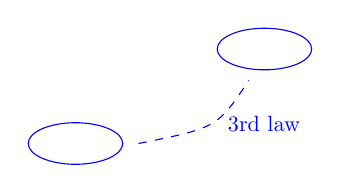
\begin{tikzpicture}[scale=.8, every node/.style={transform shape}]{r}{1}
				\draw[blue] (0,0) ellipse (0.75cm and 0.33cm);
				\draw[blue] (3,1.5) ellipse (0.75cm and 0.33cm);
				\draw[blue,dashed] (1,0) .. controls (2.25,0.25) .. (2.75,1) node[midway, right=4pt, blue] {3rd law};
			\end{tikzpicture}
	  \end{wrapfigure}
      Make a \forcediag{} for each object in each of the following situations. For each situation, circle and connect the forces that are in tandem as third law pairs, as shown.
      }
	
	\begin{enumerate}
		\item Refer to the %rocket example of \ref{fnt7.1.1-2}.
		astronaut example from \ref{14C.1}. 
		Recreate a \pchart{} and follow the instructions for the force diagram above. Explain how each of Newton's Laws can be identified in the \pcharts{} and \forcediags{}. Suppose we wanted the rocket to move at a constant speed, is a net force necessary to make this happen?
		
		\item Refer to the boat example of \ref{fnt7.1.1-3}. Recreate a \pchart{} and follow the instructions for the force diagram above. Explain how each of Newton's Laws can be identified in the \pcharts{} and \forcediags{}.
	\end{enumerate}
\end{enumerate}

\WCD

\subsection{Use Newton's Three Laws applied to a system of three objects}

\subsubsection*{\emph{Static} Case: All objects sitting still}

\begin{enumerate}
	\item Refer to the picture below of three books sitting on a table that is standing on a floor. Make a separate \forcediag{} for each of the four objects: Books~A, B, and C, and the table. The masses of the books are \unit[0.8]{kg}, \unit[0.2]{kg}, and \unit[0.5]{kg} for Books~A, B, and C, respectively and the mass of the table is \unit[30]{kg}.
	
	\begin{center}
	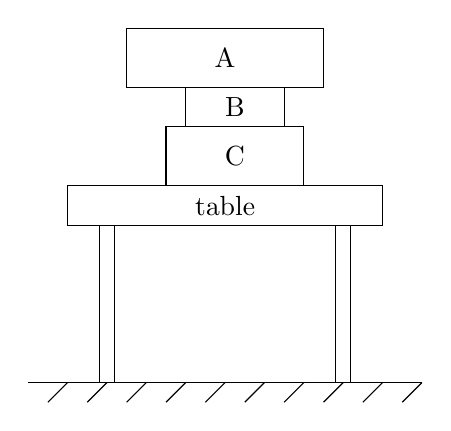
\begin{tikzpicture}{c}{1}
		% Table
		\draw[double distance = 5pt] (1,0) -- (1,2);
		\draw[double distance = 5pt] (4,0) -- (4,2);
		\draw (0.5,2) rectangle (4.5,2.5) node[midway] {table};
		% Book C
		\draw (1.75,2.5) rectangle (3.5,3.25) node[midway] {C};
		% Book B
		\draw (2,3.25) rectangle (3.25,3.75) node[midway] {B};
		% Book A
		\draw (1.25,3.75) rectangle (3.75,4.5) node[midway] {A};
		% Floor
		\draw (0,0) -- (5,0);
		\foreach \x in {0.5,1,1.5,2,2.5,3,3.5,4,4.5,5}
    			\draw (\x,0) -- (\x-0.25,-0.25);
	\end{tikzpicture}
	\end{center}
	
	\item Identify all 3rd law pairs of forces appearing in your \forcediags{} by circling the two forces and connecting as shown in the diagram on the previous page.
	
	\item Use Newton's 1st and 3rd laws to numerically determine all of the forces acting on the books and the table. If necessary, redraw your \forcediags{} so they are more to scale.
\end{enumerate}

\subsubsection*{\emph{Dynamic} Cases: Objects moving horizontally and vertically}

\begin{enumerate}
	  \setcounter{enumi}{3}
	\item If the books and table together are sliding across the room each at the same constant speed, how would your \forcediags{} change? Show precisely how it would change or explain why it would not.
	
	\item Now imagine the table is sitting in an elevator that begins to accelerate upward with an acceleration equal to $\unitfrac[2]{m}{s^2}$.
	\begin{enumerate}
		\item Make a new \forcediag{} for each book and determine the forces acting on it.
		\item Create a \pchart{} for at least two of the objects.
		\item Do any of the objects experience a net force? If so, give the magnitude and direction of each.
		\item Is it correct to say a force always equals $m\vec{a}$~?
	\end{enumerate}
\end{enumerate}

\WCD

\subsection{Applications of Newton's Laws}

\begin{fnt}
	\label{fnt8.1.1-2}

\begin{wrapfigure}{R}{0.25\textwidth}
	\vspace{-37pt}
  	\centering
	\begin{center}
	\begin{tikzpicture}[thick,scale=0.9, every node/.style={transform shape},background rectangle/.style={fill=white}, show background rectangle]
		\node[inner sep=0pt,rotate=-20] (fingers) at (-.7,4.3) {
\includegraphics[width=2cm]{pinchedFingers.png}};
		\node at (0,0) {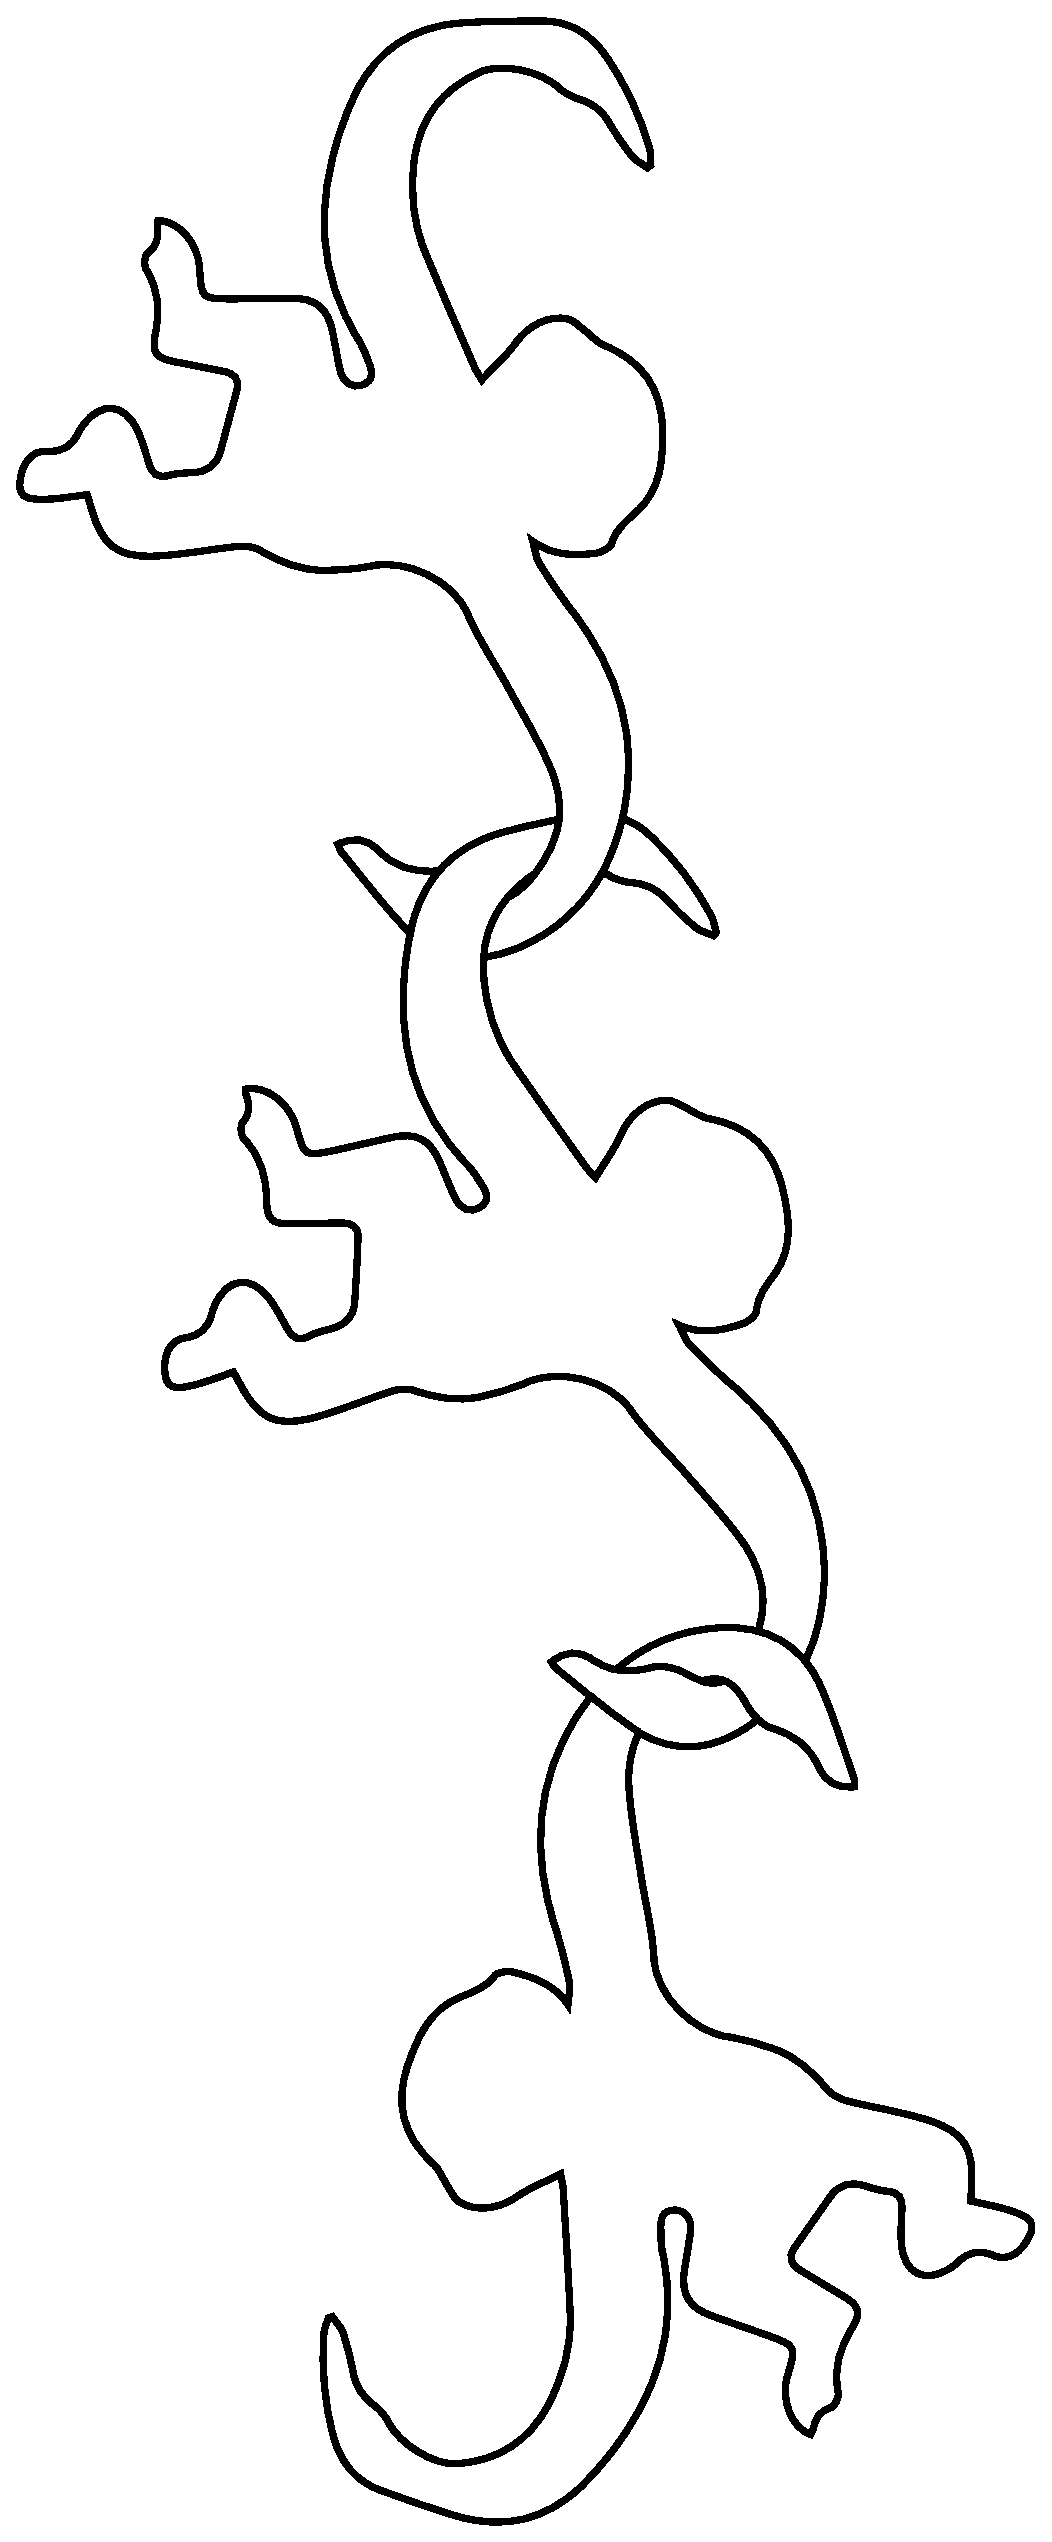
\includegraphics[width=3cm]{barrelmonkey.eps}};
		\node at (-0.25,2.4) {\scriptsize{$m=\unit[40]{g}$}};
		\node[rotate=2] at (0.12,0.1) {\scriptsize{$m=\unit[30]{g}$}};
		\node[rotate=-20] at (0.3,-2.5) {\scriptsize{$m=\unit[20]{g}$}};
	\end{tikzpicture}
	\vspace{20pt}
	\end{center}
\end{wrapfigure}

\noindent Your little brother is playing with monkeys in a barrel. The mass of each monkey is indicated in the illustration on the right. Note that your brother is holding the monkeys still and his hand weighs \unit[50]{N}.

\begin{enumerate}[(a)]
	\item Make a separate \forcediag{} for each of the four objects, the hand, top monkey, middle monkey, bottom monkey.
	
	\item Identify all 3rd law pairs of forces appearing in your \forcediags{} by circling the two forces and connecting them with a line.
	
	\item Use Newton's 1st and 3rd laws to numerically determine all of the forces acting on the monkeys and the hand. If necessary, redraw your \forcediags{}, so they are more to scale.
\end{enumerate}
\end{fnt}

\vspace{-6pt}
\WCD
\vspace{12pt}

%\section{Some things to ponder before we begin}
\label{act8.1.0-part2}

\begin{fnt}
	\label{fnt8.1.0-2}

We've already investigated this problem with one spring scale in \ref{8.1.0-1}. Now, imagine you have two spring scales, A and B, connected at the end of the scale that doesn't move. The end that moves of each spring scale (where you take readings from) is attached to a string that goes over a pulley and connects to a \unit[1]{kg} mass for both spring scales A and B.

\vspace{-6pt}
\begin{center}
	\begin{tikzpicture}[thin,scale=.7, every node/.style={transform shape},background rectangle/.style={fill=white}, show background rectangle]
		%table
		\draw (2,3) rectangle (10,3.5);
		\draw (3,0) rectangle (3.25,3);
		\draw (8.75,0) rectangle (9,3);
		%pulleys
		\draw (1.5,3.62) circle (.3);
		\draw (10.5,3.62) circle (.3);
		\filldraw[fill=white,draw=black] (1.5,3.5) rectangle (2.5,3.7);
		\filldraw[fill=white,draw=black] (9.5,3.5) rectangle (10.5,3.7);
		%weights
		\draw (.8,1.5) rectangle (1.6,2) node[midway] {\unit[1]{kg}};
		\draw (10.4,1.5) rectangle (11.2,2) node[midway] {\unit[1]{kg}};
		%string
		\draw (1.2,2) -- (1.2,3.62);
		\draw (10.8,2) -- (10.8,3.62);
		\draw (1.5,3.92) -- (4.5,3.92);
		\draw (10.5,3.92) -- (7.7,3.92);
		%spring scales
		\draw (4.9,3.72) rectangle (5.9,4.12) node[midway,above=6pt,align=center] {\scriptsize{Spring}\\[-1.2ex]\scriptsize{Scale A}};
		\foreach \x in {5.1, 5.3, 5.5, 5.7}
			\draw (\x,3.8) -- (\x,4.04);
		\draw (6,3.92) circle (.1);
		\draw (4.7,3.92) ellipse (.2 and .1);
		\draw (6.3,3.72) rectangle (7.3,4.12) node[midway,above=6pt,align=center] {\scriptsize{Spring}\\[-1.2ex]\scriptsize{Scale B}};
		\foreach \x in {6.5, 6.7, 6.9, 7.1}
			\draw (\x,3.8) -- (\x,4.04);
		\draw (6.2,3.92) circle (.1);
		\draw (7.5,3.92) ellipse (.2 and .1);
	\end{tikzpicture}
\end{center}
\vspace{-24pt}

\begin{enumerate}[(a)]
	\item State what you think \emph{each} spring scale will read in this situation.
	
	\item Construct a logical argument that explains why the spring scales read what you reported in Question~(a). You should treat this as a quiz/test question and therefore use complete sentences, reference any models you think will strengthen your argument, and provide evidence to support your claim.
\end{enumerate}
\end{fnt}

\vspace{-6pt}
\WCD

%We'll skip this one...
%\begin{fnt}
%	\label{fnt8.1.1-3}

Use Newton's laws to analyze the three car train shown in the picture. Car~A is the engine and pulls Cars~B and C. Car~A has a mass of \unit[10000]{kg}, Car~B is \unit[8000]{kg}, and Car~C is \unit[5000]{kg}. The train is initially at rest but then starts to move with an acceleration of $\unitfrac[3]{m}{s^2}$ to the left.

Calculate the force of Car~B on Car~A. Answer the following questions to help you do this.

\begin{enumerate}[(a)]
	\item Draw a \forcediag{} for EACH car with the train at rest.

	\item Car~A powers up its engine and each car starts to accelerate. What provides the force for Car~C to start accelerating?

	\item Draw a \forcediag{} for each car now that each car is accelerating (You may need to come back and update them after you determine the numerical values for each force).

	\item Calculate the force of Car~B on Car~C. 
		
		\textbf{Hint:} the sum of the forces on EACH car is equal to the mass of that car times the car's acceleration. $\sum \vec{F}_A = m_A \vec{a}_A$.
	
	\item What is the net force on Car~B?
	
	\item Calculate the force of Car~A on Car~B.
	
	\item What is the force of Car~B on Car~A?
	
	\item What is the magnitude and direction of the force of the rails on Car~A?
\end{enumerate}
%\end{fnt}

%\WCD

%\begin{fnt}
%	\label{fnt8.1.1-4}

For each of the following
\begin{enumerate}[(i)]
	\item Identify all the forces acting on the object of interest (\textbf{\em bold} in each statement) in each of the situations below.
	
	\item Draw a \forcediag{} for the object of interest.
	
	Note: Be sure to label your force vectors and make their length approximately equal to their magnitudes.
\end{enumerate}

\begin{enumerate}[(a)]
	\item The \textbf{\em softball player} is slowing as she slides into the base.
	\item The \textbf{\em child} on the swing who is being pulled back before being released.
	\item A \textbf{\em skydiver} who is descending at a constant velocity.
	\item The \textbf{\em squirrel} that is sitting still on a slanted roof.
\end{enumerate}
%\end{fnt}
%
%\WCD